\documentclass[12pt]{article}

% Margins
\usepackage[letterpaper, margin=1in]{geometry}
\usepackage{xcolor}
\usepackage{color}
\usepackage{fancyvrb}
\usepackage{hyperref}
\usepackage{longtable}
\usepackage{multicol}
\usepackage{tabu}
\usepackage{booktabs}
\usepackage{graphicx}
\usepackage{amsmath,amssymb}
\usepackage{subcaption}
\usepackage[hyperref=true,backend=biber,sorting=none,backref=true]{biblatex}

% Font
\usepackage{times}

\addbibresource{cite.bib}

% Title
\title{Comparing Gibbs sampling and EM-Algorithm method for missing data imputation}
\author{Hao Xu T00732492}
\date{\today}

\begin{document}

\maketitle

\begin{abstract}

This study presents a comparative analysis of Gibbs sampling methods and the Expectation-Maximization (EM) Algorithm for imputing missing data, specifically within the context of an IELTS scores dataset assumed to follow a multivariate normal distribution. Through implementation and simulation in R, we evaluated the efficacy of both techniques across varying levels of data incompleteness. Our findings reveal that both Gibbs sampling and the EM Algorithm demonstrate comparable performance when the proportion of missing data is minimal. However, as the extent of missing data increases to 30\%, Gibbs sampling outperforms the EM Algorithm in terms of imputation accuracy and reliability. These results underscore the potential of Gibbs sampling as a robust method for handling larger proportions of missing data, providing significant implications for researchers and practitioners dealing with incomplete datasets in educational assessments and beyond.

\end{abstract}

\section{Introduction}

Missing data imputation is a critical process in data analysis across various fields, addressing the challenge of incomplete datasets which can potentially lead to biased or invalid conclusions if not properly handled. In the real world, missing data occur in virtually every domain including healthcare, finance, social sciences, and environmental studies. For instance, in healthcare, missing data can arise from patient dropout, non-response to surveys, or malfunctioning equipment, leading to incomplete patient records that are crucial for accurate diagnosis and treatment planning. Similarly, in finance, gaps in datasets can affect the analysis of economic trends or financial risk assessments, where every data point might represent crucial information about market behaviors or credit scores. Imputation techniques, such as the EM algorithm, enable researchers and analysts to estimate these missing values accurately, thereby maintaining the integrity of statistical analyses and ensuring that decision-making is based on robust and comprehensive data sets. This not only enhances the quality of insights derived from data but also supports more informed policy-making and strategic planning in professional practices.

\section{Literature Review}
% Literature review content goes here

\subsection{Gibbs sampling method}

Gibbs Sampling, introduced in 1984 by Geman and Geman \cite{Geman1984}, is a form of Markov chain Monte Carlo (MCMC) methodology that facilitates the simulation from a joint probability distribution. The process involves sequentially sampling from the conditional distributions of each variable, holding the values of all other variables at their current states. This technique is particularly useful in the context of missing data imputation, where Gibbs sampling is employed to generate samples of the missing data based on their conditional distributions, given the observed data and the current estimates of parameters. This iterative approach ensures a comprehensive exploration of the distribution, making it a powerful tool for dealing with incomplete datasets in statistical analysis.

\subsection{EM algorithm}

The Expectation-Maximization (EM) algorithm, proposed in 1977 by Arthur P. Dempster \cite{Dempster1977}, is a hybrid inferential method that straddles both Bayesian and frequentist statistical frameworks. While primarily a maximum likelihood approach, EM yields both a probability distribution over latent variables—reminiscent of Bayesian analysis—and a point estimate for the parameter $\theta$, which could be either a maximum likelihood estimate or a posterior mode. In cases where a fully Bayesian treatment is desirable, $\theta$ can be treated as an additional latent variable, effectively integrating it within the entire probabilistic model. Under such a Bayesian extension, the traditional separation of the algorithm into Expectation (E) and Maximization (M) steps becomes less distinct, showcasing the fluidity and adaptability of the EM algorithm in handling incomplete data sets across various statistical paradigms.

\subsection{Missing data imputation}

In statistical analysis, understanding the nature of missing data is crucial for applying appropriate imputation methods and interpreting results accurately. Missing data can be classified into three primary types: Missing Completely at Random (MCAR), Missing at Random (MAR), and Missing Not at Random (MNAR). 

\paragraph{Type 1: Missing Completely at Random (MCAR)}

Missing Completely at Random (MCAR) refers to data that is absent purely due to random factors, with no discernible pattern or structure influencing its absence. In such cases, the missing data points are independent of both the observed and unobserved data.

\paragraph{Type 2: Missing at Random (MAR)}

Missing at Random (MAR) occurs when the absence of data is related to the observable attributes of the data set. Although the missing data itself isn't random, its likelihood can be accurately predicted using other available information or variables within the same observation.

\paragraph{Type 3: Missing Not at Random (MNAR)}

Missing Not at Random (MNAR) describes a scenario where the missing data is directly influenced by the values that are missing. This type of missing data possesses inherent patterns that are closely linked to the characteristics of the missing observations themselves. Failure to accurately identify and address MNAR can lead to biased analyses and less effective solutions when applied in real-world contexts.

In this paper, we are only considering Type 1 and Type 2 case. In cases where the data are missing but not at random, we need to model the relationship between the missing data and the parameters\cite{Gelman2013}, which makes comparison betweenn EM algorithms and Gibbs samplign methods complicated.

\section{Objectives}

The primary objectives of this study are outlined as follows:

\begin{enumerate}
	\item \textbf{Implement the EM-Algorithms and Gibbs sampling methods in R.}
Our first goal is to develop and implement robust computational procedures for both the EM Algorithm and Gibbs sampling methods using the R programming language. This implementation will involve writing custom functions and scripts to handle missing data imputation processes efficiently. By leveraging R’s powerful statistical and graphical capabilities, we aim to create a flexible framework that can be applied to a wide range of datasets with missing values.
	\item \textbf{ Identify the assumptions of applying these two methods.}
Both the EM Algorithm and Gibbs sampling rely on specific statistical assumptions which must be clearly understood and validated to ensure the appropriateness of each method for handling missing data. This objective involves a thorough examination of the underlying assumptions such as data distribution (e.g., assuming multivariate normality), independence, and the missing data mechanism (MCAR, MAR, MNAR). Recognizing these assumptions will aid in the proper application and interpretation of each technique's results.
\item \textbf{Comparative Analysis of Performance.}
The final objective is to conduct a detailed comparison of the performance of the EM Algorithm and Gibbs sampling across various scenarios characterized by different percentages of missing data. Performance metrics such as imputation accuracy, computational efficiency, and the robustness of each method will be evaluated. This comparison will not only focus on scenarios with minimal missing data (e.g., 5-10\%) but also explore the efficacy of both methods under substantial missing conditions (up to 30\% and beyond). The insights gained from this analysis will guide practitioners in choosing the most suitable method based on the extent and nature of missing data in their specific contexts.
\end{enumerate}


\section{Data and Variables}

In this work, we downloaded the data from 2019 IELTS Test Statistic Report\footnote{\url{https://ieltscenterofficial.github.io/examcenter/for-researchers/test-statistics/test-taker-performance.html}} and extracted the ``Academic mean performance by nationality" table.

The table contains five columnns, which are ``Reading", ``Listening", ``Writing", ``Speaking" and ``Overall", each represent one type of score from the IELTS test. Each row of the data represent the average score of students from a specific nationality. Figure~\ref{fig:IELTS} (in Appendix) plots all the data poins from the table.

The univariate histogram and bivariate scatterplots of the test data is shown in Figure~\ref{fig:stats}. We can see that all five variabels are normally distributed, and there are correlation between these 5 variables. So our assumption is that the data follows a multivariate normal distribution.

\begin{figure}[htpb]
	\centering
	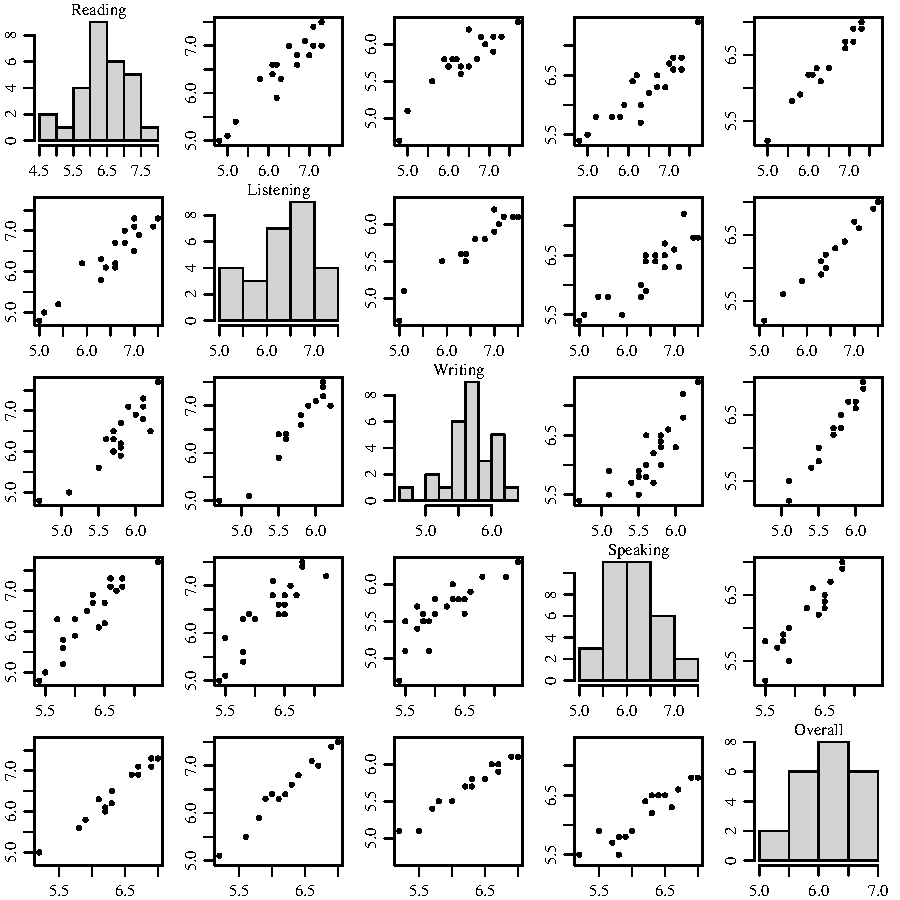
\includegraphics[width=0.6\textwidth]{pic/stat.pdf}
	\caption{IELTS scores of 40 different nationalities}
	\label{fig:stats}
\end{figure}

\section{Methods}

This section outlines the methodologies employed to simulate the missing data imputation preocess in the IELTS scores dataset. Specifically, we apply Gibbs Sampling and the EM Algorithm, both robust methods in the field of statistical imputation, to estimate missing values under the assumption that the data follows a multivariate normal distribution. The objective is to not only impute missing values but also to compare the efficacy and computational efficiency of these two approaches under varying conditions of data incompleteness. This comparative analysis aims to identify which method provides more accurate imputations and under what circumstances.

\subsection{Gibbs sampling}
\label{Gibbs}

In Bayesian inference we treat the unknown parameters of interests as random variables. Assuming multivariate normal model, the parameters $\boldsymbol{\theta}$ and $\Sigma$ are unknown, and the missing data are also an unknown. Further more, the missing data are also key compoents of our model. 
Treating it as such allows us to use Gibbs sampling to make inference on $\boldsymbol{\theta}$, $\Sigma$, as well as to make predictions for the missing values.\cite{Hoff2009}

Let $\mathbf{Y}$ be the $n\times p$ matrix of all IELTS scores, observed and unobserved, and let $O$ be the $n \times p$ matrix in which $o_{i,j} = 1$ if $Y_{i,j}$ is observed and $o_{i,j} = 0$ if $Y_{i,j}$ is missing. The matrix $\mathbf{Y}$ can then be thought of as consisting of two parts:

\begin{itemize}
\item $\mathbf{Y}_{\text{obs}} = \{y_{i,j}: o_{i,j} = 1\}$, the data that we do observe, and
\item $\mathbf{Y}_{\text{miss}} = \{y_{i,j}: o_{i,j} = 0\}$, the data that we do not observe.
\end{itemize}

Prior selection: we take the mean of the observed data as the prior mean $\boldsymbol{\mu}_0$. For standard deviation, we want to use a weak prior. From the IELTS test statistics report\footnote{\url{https://ielts.org/researchers/our-research/test-statistics}}, we know that the more than 95\% people have a test score between 4 and 8.5. Therefore, we know that given the mean $\boldsymbol{\mu}_0$, we have the following property: 
\[
\Phi(\frac{\mathbf{8.5}-\boldsymbol{\mu}_0}{\boldsymbol{\sigma}_0})-\Phi(\frac{\mathbf{4}-\boldsymbol{\mu}_0}{\boldsymbol{\sigma}_0}) = (95\%,95\%,95\%,95\%,95\%)^{T}
\] 

In practice, we do not have to solve the above equation precisely. Instead, we take all standard deviation elemennts in $\boldsymbol{\sigma}_0 = \frac{8-4.5}{2*\text{qnorm}(0.95)} = 1.1538$. Also we know that there are some correlations between the four sections and overall scores of IELTS test, so we take the prior variance-covariance matrix as follows:
\[
\Lambda_0 = \Sigma^{(0)} = \begin{pmatrix} 
1.33&0.67&0.67&0.67&0.67\\
0.67&1.33&0.67&0.67&0.67\\
0.67&0.67&1.33&0.67&0.67\\
0.67&0.67&0.67&1.33&0.67\\
0.67&0.67&0.67&0.67&1.33\\
\end{pmatrix} 
.\] 

Given the starting values $\{\Sigma^{(0)}, \mathbf{Y}_\text{miss}^{(0)}\}$, we iteratively generate $\{\boldsymbol{\theta}^{(s+1)}, \Sigma^{(s+1)}, \mathbf{Y}_{\text{miss}}^{(s+1)}\}$ from $\{\boldsymbol{\theta}^{(s)}, \Sigma^{(s)}, \mathbf{Y}_{\text{miss}}^{(s)}\}$ by the following steps:

\begin{enumerate}
\item sampling $\boldsymbol{\theta}^{(s+1)}$ from $\text{multivariate normal}(\boldsymbol{\mu}_n, \Lambda_n)$, where 
\begin{align*}
\boldsymbol{\mu}_n &= (\Lambda_0^{-1}+n{\Sigma^{(s)}}^{-1})^{-1}(\Lambda_0^{-1}\boldsymbol{\mu}_0+n{\Sigma^{(s)}}^{-1}\overline{\boldsymbol{Y}^{(s)}}) \text{ and}\\
\Lambda_n &= (\Lambda_0^{-1}+n{\Sigma^{(s)}}^{-1})^{-1}
\end{align*}
\item sampling $\Sigma^{(s+1)}$ from invert-Wishart $(\nu_0+5, \mathbf{S}_n^{-1})$, where 
\begin{align*}
\mathbf{S}_n &=  \mathbf{S}_0+\mathbf{S}_\theta\\
\mathbf{S}_0 &= \Lambda_0\\
\mathbf{S}_\theta &= \sum_{i=1}^{n} (\mathbf{Y}_i^{(s)}-\boldsymbol{\theta}^{(s+1)})(\mathbf{Y}^{(s)}_i-\boldsymbol{\theta}^{(s+1)})^T\text{ and}\\
\nu_0 &= 2\text{ for a weak prior}
\end{align*}
\item sampling $\mathbf{Y}_{\text{miss}}^{(s+1)}$ from multivariate normal $(\boldsymbol{\theta}^{(s+1)}_{b|a}, \Sigma^{(s+1)}_{b|a})$, where
\begin{align*}
\boldsymbol{\theta}^{(s+1)}_{b|a} &= \boldsymbol{\theta}^{(s+1)}_{[b]} + \Sigma^{(s+1)}_{[b,a]}(\Sigma^{(s+1)}_{[a,a]})^{-1}(\mathbf{Y}_{[a]} - \boldsymbol{\theta}^{(s+1)}_{[a]})\\
\Sigma^{(s+1)}_{b|a} &= {\Sigma}^{(s+1)}_{[b,b]} + \Sigma^{(s+1)}_{[b,a]}(\Sigma^{(s+1)}_{[a,a]})^{-1}\Sigma^{(s+1)}_{[a,b]}.
\end{align*}
Here, $\boldsymbol{\theta}^{(s+1)}_{[b]}$ refers to the elements of $\boldsymbol{\theta}^{(s+1)}$ corresponding to the indices in $\mathbf{b}$. $\mathbf{b}$ is a subset of variable indices $\{1,2,3,4,5\}$ whose corresponding variable $Y$ is missing and  $\mathbf{a}$ is a complement of $\mathbf{b}$. $\Sigma_{[a,b]}$ refers to the matrix made up of the elemennts that are in rows $\mathbf{a}$ and column $\mathbf{b}$ of $\Sigma$.

\end{enumerate}

\subsection{EM algorithm}

Under the same setup of a multivariate normal model for the IELTS Scores data $\mathbf{Y}$ as described in section~\ref{Gibbs}, we derive the steps for EM algorithm in this section. 

The general idea to perform EM algorithm is to iterate through the following steps until apparent convergence\cite{Roderick2020}:
\begin{enumerate}
\item Replace missing values by estimated values
\item Estimate parameters 
\item Re-estimate the missing values assuming the new parameter estimates are correct
\item Re-estimate parameters
\end{enumerate}

In EM algorithm, we do not treat $\boldsymbol{\theta}$ and $\Sigma$ as a random variable as in section~\ref{Gibbs}. Instead, when estimating those parameters, we are trying to maximize the loglikelihood function:
\[
\mathcal{L}(\boldsymbol{\theta}, \Sigma|\mathbf{Y}_{\text{obs}}) = \text{Const} - \frac{1}{2}\sum_{i=1}^{n} \ln \mid \Sigma_{[a,a]} \mid -\frac{1}{2}\sum_{i=1}^{n} (\mathbf{Y}_{i,[a]} - \boldsymbol{\theta}_{[a]})^T\Sigma_{[a,a]}(\mathbf{Y}_{i,[a]} - \boldsymbol{\theta}_{[a]})
.\] 

Here we are continue using the notation defined in section~\ref{Gibbs} step 3, where $\boldsymbol{\theta}_{[a]}$ and $\Sigma_{[a,a]}$ represent the mean and variance-covariance matrix of the observed values respectively.

The hypothetical distribution of the complete data $\mathbf{Y}$ is a multivariate normal which belongs to the regular exponential family, therefore it has the following sufficient statistics:
\[
S = \left( \sum_{i=1}^{n} y_{i,j};\text{ and } \sum_{i=1}^{n} y_{i,j}y_{i,k},\quad j,k=1,2,3,4,5\right) 
.\] 

The EM algorithm is to iteratively run through the following steps until convergence: (Using $\boldsymbol{\theta}^{(t)}\text{ and } \Sigma^{(t)}$ to represent the estimates of the parameters at the $t^{\text{th}}$ iteration of EM )

\begin{enumerate}
	\item The E step of the EM algorithm for iteration $t+1$ is to calculate
\begin{enumerate}
	\item $E\left( \sum_{i=1}^{n} y_{i,j}|\mathbf{Y}_{\text{obs}}, \boldsymbol{\theta}^{(t)} \right) = \sum_{i=1}^{n} y_{i,j}^{(t+1)}, j=1,2,3,4,5$ and
	\item $E\left( \sum_{i=1}^{n} y_{i,j}y_{i,k}|\mathbf{Y}_{\text{obs}}, \boldsymbol{\theta}^{(t)} \right) = \sum_{i=1}^{n} \left( y_{i,j}^{(t+1)}y_{i,k}^{(t+1)}+c_{j,k,i}^{(t+1)} \right) , j,k=1,2,3,4,5$
	\item sampling $\mathbf{Y}_{\text{miss}}$ from multivariate normal $\left( \boldsymbol{\theta}_{b|a}^{(t)},  \Sigma_{b|a}^{(t)} \right) $ (same calculation as step 3 in the Gibbs sampling method)
\end{enumerate}
Here in the above steps,
\[
y_{i,j}^{(t+1)} = \begin{cases}
	y_{i,j} &,\text{if } o_{i,j} = 1,\\
	E\left( y_{i,j}| \mathbf{Y}_{i,[a]}, \boldsymbol{\theta}^{(t)}\right) &,\text{if } o_{i,j} = 0
\end{cases}
\] and
\[
c_{j,k,i}^{(t+1)} = \begin{cases}
0	&,\text{if } o_{i,j} + o_{i,k} \geq 1,\\
\text{Cov}(y_{i,j}, y_{j,k}|\mathbf{Y}_{i,[a]}, \boldsymbol{\theta}^{(t)}) &,\text{if } o_{i,j} + o_{i,k} = 0,\\
\end{cases}
\]
\item The M step is to update $\boldsymbol{\theta}^{(t+1)}$ and $\Sigma^{(t+1)}$ based on the result from the E step. 
\begin{enumerate}
	\item The $j^{th}$ element at $\boldsymbol{\theta}^{(t+1)}$ is: $\theta_j^{(t+1)} = n^{-1}E\left( \sum_{i=1}^{n} y_{i,j}|\mathbf{Y}_{\text{obs}}, \boldsymbol{\theta}^{(t)} \right), j=1,2,3,4,5$
\item The element at $j^{th}$ row $k^{th}$ column of $\Sigma^{(t+1)}$ is denoted by $\sigma_{j,k}^{(t+1)}$ 
\[
\sigma_{j,k}^{(t+1)} = n^{-1} E\left( \sum_{i=1}^{n} y_{i,j}y_{i,k}|\mathbf{Y}_{\text{obs}}, \boldsymbol{\theta}^{(t)} \right) - \theta_j^{(t+1)}\theta_k^{(t+1)},\qquad j,k=1,2,3,4,5
\] 
\end{enumerate}
\item Calculate $\|\boldsymbol{\theta}^{(t+1)} - \boldsymbol{\theta}^{(t)}\|$ and $\|\Sigma^{(t+1)}-\Sigma^{(t)}\|$ to check for convergence.
\end{enumerate}

%See pdf 262 page chapter 11.2.1 of \cite{Roderick2020} for details.

\section{Simulations}

To simulate missing data within our dataset, we employ the \texttt{rbinom(n*p,1,.9)} function in R, which randomly assigns \texttt{NA} (i.e., missing data status) to selected data entries. The probability parameter pp is varied to create different scenarios with missing data ranging from 10\% to 30\%. This approach allows us to maintain a control group by keeping a record of the true values for subsequent performance evaluation.

In the simulation of the EM algorithm, we configure the maximum number of iterations to 100 and set the convergence threshold to $10^{-6}$. The outcomes of these simulations include the estimation of the final mean and variance-covariance matrix, as well as the imputation of missing data.

For the Gibbs sampling process, we choose a longer iteration count, set at 1000 iterations. This approach aims to generate robust estimates of the posterior mean, variance-covariance matrix, and the imputed missing data. The extended number of iterations in Gibbs sampling is expected to provide more accurate and stable results, especially in scenarios with higher percentages of missing data.

The effectiveness of each method is assessed by computing the mean square error (MSE) of the predictions across the various scenarios of missing data percentages, thus providing a quantitative measure of performance.

\section{Results}

In this section, we present the findings from our simulations to evaluate the performance of Gibbs Sampling and the EM Algorithm in handling missing data within an IELTS scores dataset. To facilitate a clear and comprehensive understanding of how well each method predicted the missing values, we have included a detailed plot that illustrates the correlation between the predicted values and the true values. This plot can be found in the Appendix (see Appendix~\ref{sim-result}).

Furthermore, to quantitatively assess the accuracy of each imputation method across different scenarios, we calculated the mean squared errors (MSE) for varying levels of missing data. These MSE values are crucial indicators of prediction accuracy, providing a straightforward metric for comparing the performance of the two methods under conditions ranging from 10\% to 30\% missing data. 

The mean squared errors for each scenario are listed in Table~\ref{tab:mse_comparison}.

\begin{table}[h]
\centering
\begin{tabular}{ccc}
\hline
\textbf{Percentage Missing} & \textbf{EM Algorithm MSE} & \textbf{Gibbs Sampling MSE} \\
\hline
10\% & 0.036 & 0.015 \\
15\% & 0.026 & 0.024 \\
20\% & 0.017 & 0.022\\
25\% & 0.033 & 0.027 \\
30\% & 0.069 & 0.039\\
\hline
\end{tabular}
\caption{Comparison of Mean Squared Errors for EM Algorithm and Gibbs Sampling}
\label{tab:mse_comparison}
\end{table}

We also recoreded the computation time it takes to run each algorithms, listed in Table~\ref{tab:time_comparison}

\begin{table}[h]
\centering
\begin{tabular}{cc}
\hline
\textbf{EM Algorithm} & \textbf{Gibbs Sampling} \\
\hline
0.6542037 & 11.12866 \\
1.000516 & 10.44828 \\
1.118946 & 10.67758 \\
1.15855 & 10.25005 \\
1.262844 & 10.27943 \\
\hline
\end{tabular}
\caption{Comparison of computation time (in seconds) for EM Algorithm and Gibbs Sampling}
\label{tab:time_comparison}
\end{table}
\section{Summary and Discussions}

From the simulation results, we observe that both the Gibbs sampling method and the EM algorithm perform competently in the task of missing data imputation. When the amount of missing data is relatively low (up to 20\%), the performance of both methods is comparable. Notably, the EM algorithm demonstrates a significantly shorter computation time, requiring approximately one-tenth the computation duration needed for Gibbs sampling.

However, the scenario changes as the missing data proportion increases to 30\%. In such cases, Gibbs sampling notably surpasses the EM algorithm in terms of prediction accuracy. This superior performance of Gibbs sampling in high-missing-data contexts suggests that Bayesian methods provide a robust framework for dealing with complex uncertainty and integrating prior knowledge effectively. These methods are particularly adept at handling larger gaps in data by utilizing probability distributions to estimate missing values, rather than relying solely on observed data patterns. This approach can be particularly beneficial in scenarios where traditional methods might fail to provide reliable estimates due to the extent of incompleteness. Thus, Bayesian techniques like Gibbs sampling demonstrate considerable potential in improving the quality of data imputation in statistical analyses, especially when the missing data proportion is substantial.

These findings suggest that while the EM algorithm might be preferred for quicker imputation tasks with less missing data, Gibbs sampling emerges as the more robust method in scenarios where the missing data proportion is substantial and precision is paramount. Future research could explore the scalability of these methods in even larger datasets and the potential adjustments in their configurations to optimize performance across varying conditions.

\printbibliography
% References content goes here

\newpage

\section{Appendix}
% Appendix content goes here
\subsection{IELTS Scores of each Nationality}
\begin{figure}[htpb]
	\centering
	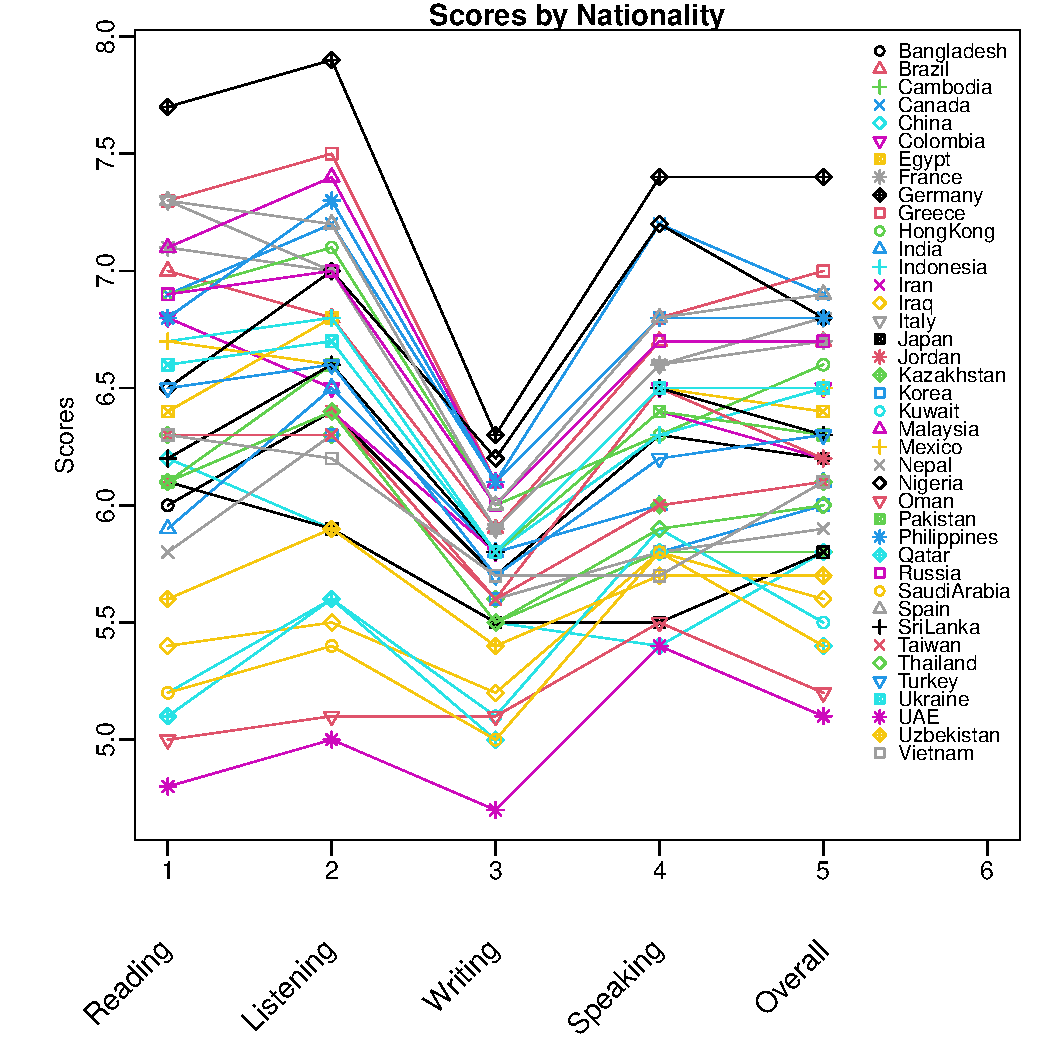
\includegraphics[width=0.8\textwidth]{pic/IELTS.pdf}
	\caption{IELTS Scores of each Nationality}
	\label{fig:IELTS}
\end{figure}


\subsection{Simulation result:}
\label{sim-result}
\newpage
\subsubsection{10\% of missing data}
\begin{figure}[h!]
\centering
\begin{subfigure}{0.4\textwidth}
    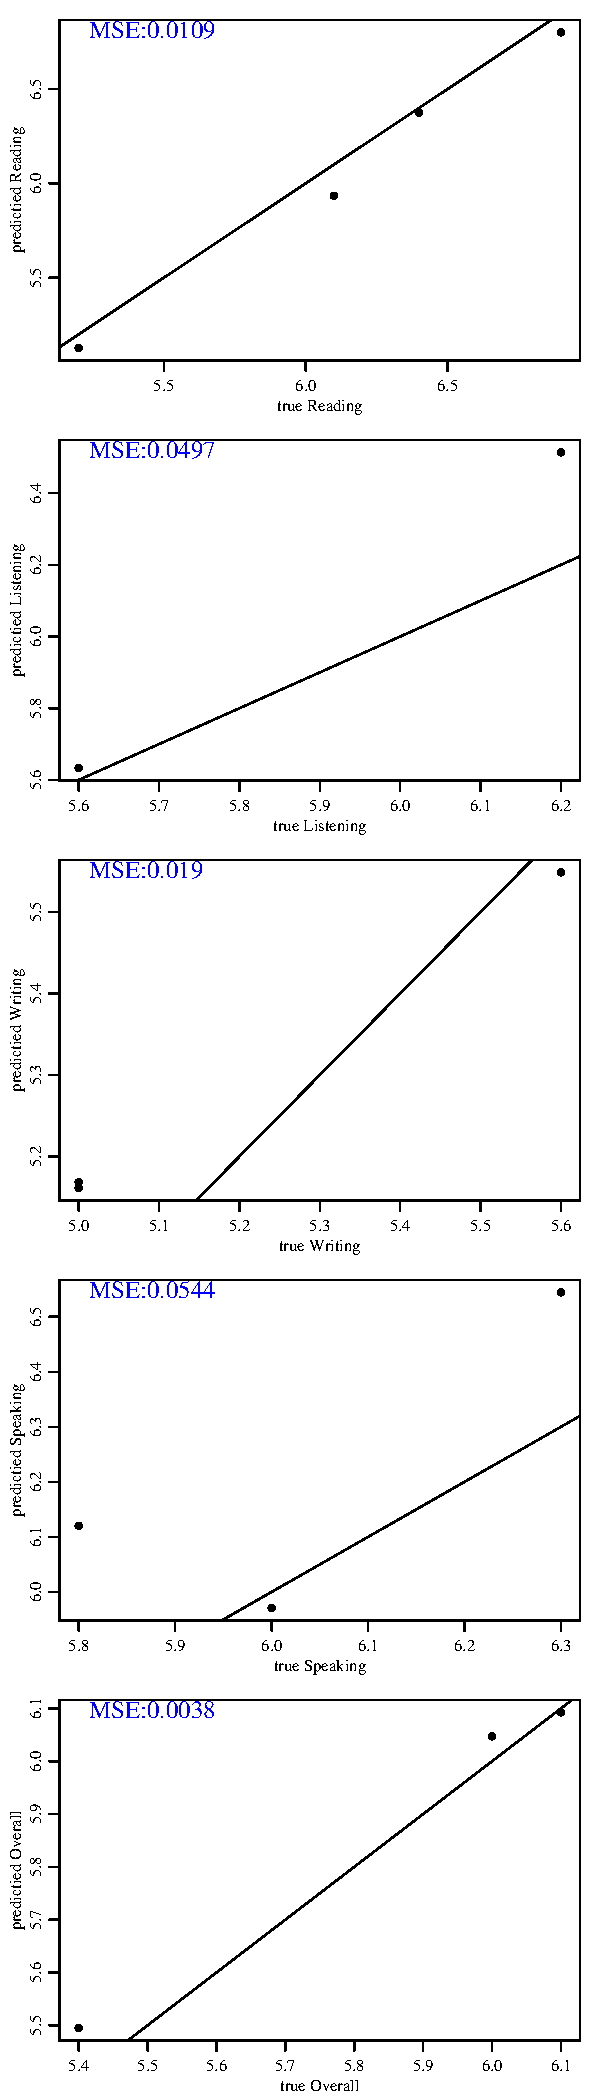
\includegraphics[height=.85\textheight]{pic/0.10/EM_PredvsTrue.pdf}
    \caption{EM algorithm}
    \label{fig:0.1-empvt}
\end{subfigure}
%\hfill
\begin{subfigure}{0.4\textwidth}
    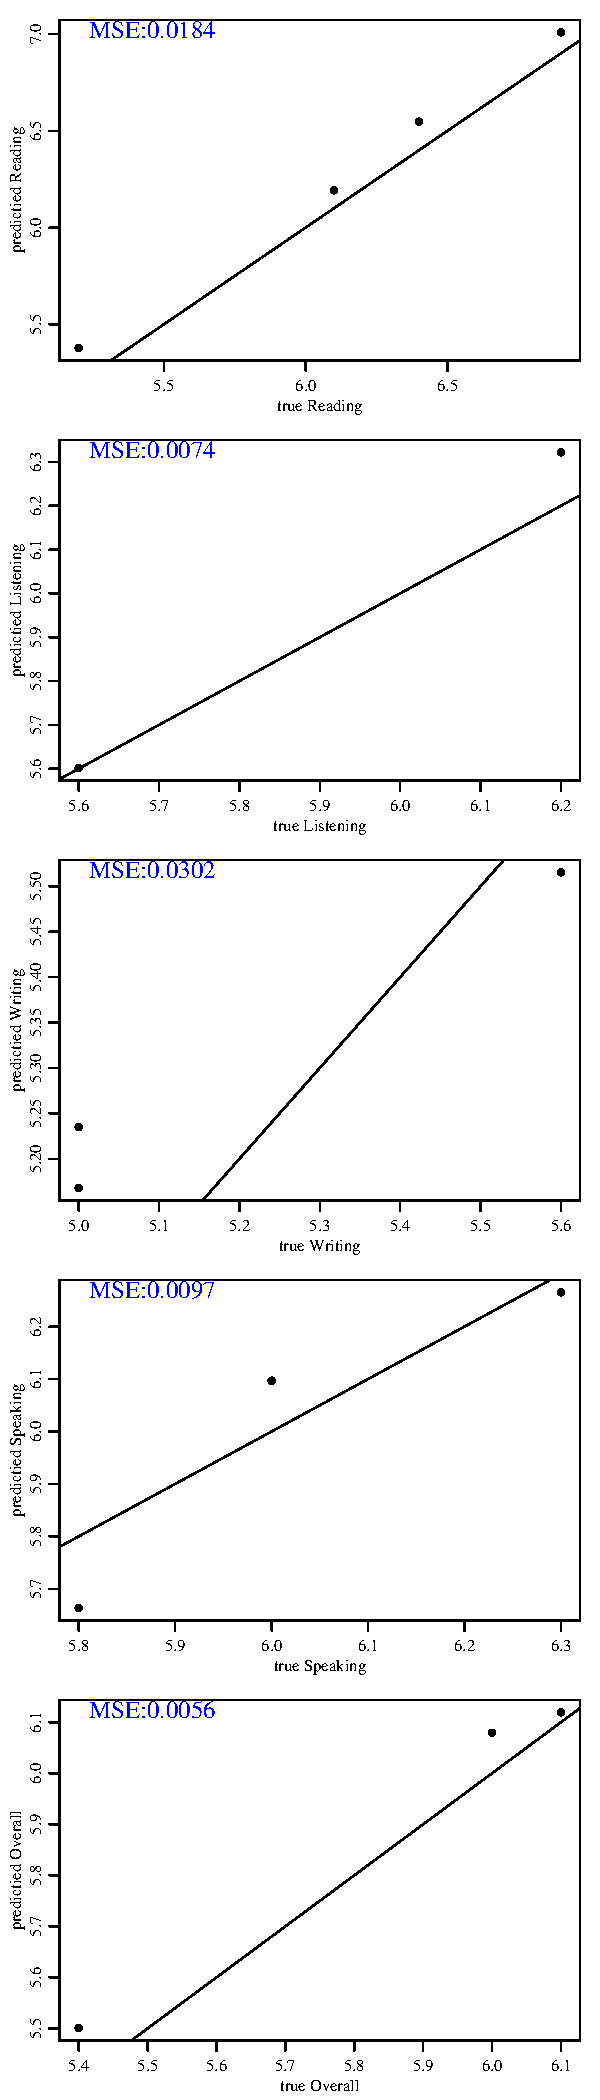
\includegraphics[height=.85\textheight]{pic/0.10/Gibbs_PredvsTrue.pdf}
    \caption{Gibbs sampling method}
    \label{fig:0.1-gibbspvt}
\end{subfigure}
        
\caption{Prediction vs True value}
\label{fig:0.1-pvt}
\end{figure}

\begin{figure}[htbp]
	\centering
	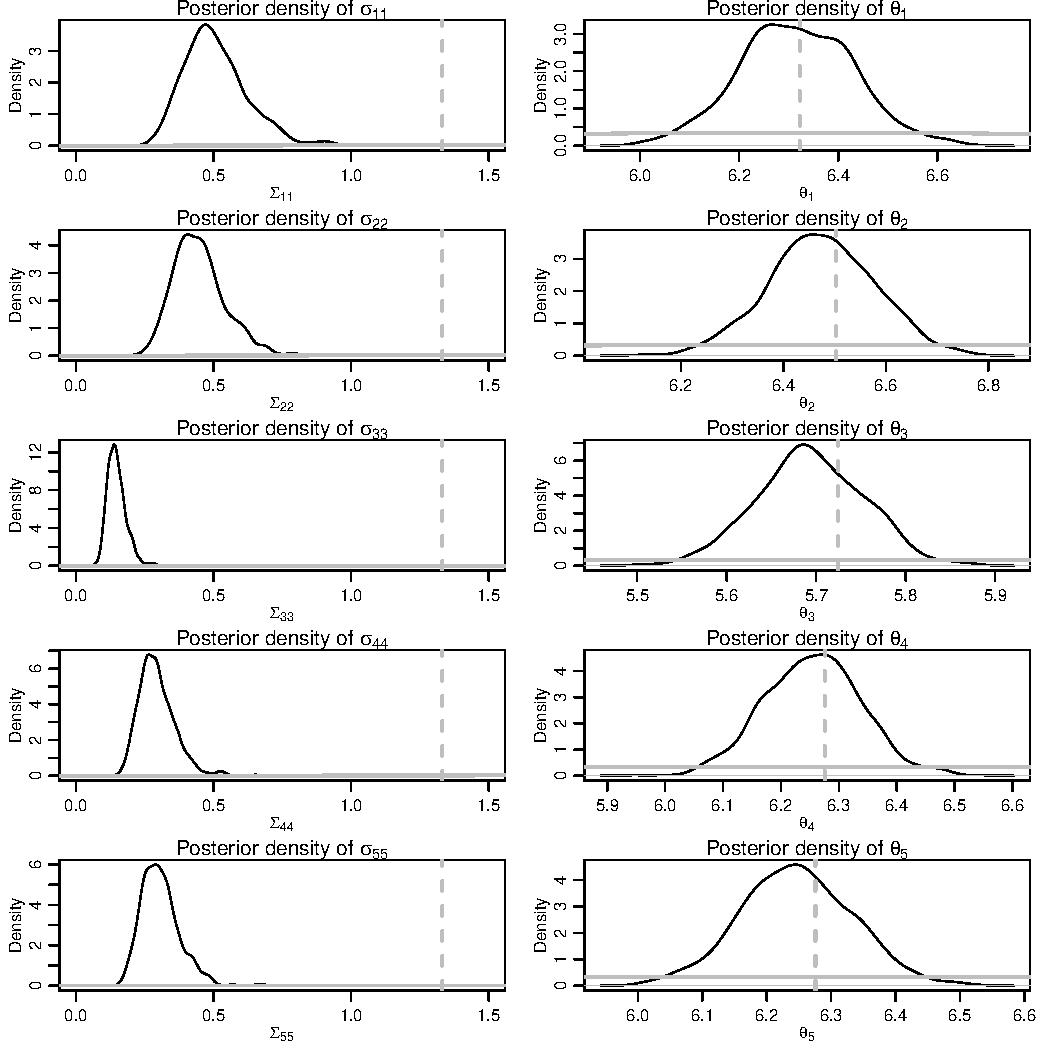
\includegraphics[width=.85\textwidth]{pic/0.10/Posterior_vs_Prior.pdf}
	\caption{The posterior (and prior) distribution of $\sigma_{j, j}$ (left) and $\theta_j$ (right). Posterior distribution is ploted in black, and prior distribution is ploted in gray. The vertical dashed line marks the initial value for prior.}
	\label{fig:0.1-Posterior_vs_Prior}
\end{figure}
\newpage
\subsubsection{15\% of missing data}
\begin{figure}[h!]
\centering
\begin{subfigure}{0.4\textwidth}
    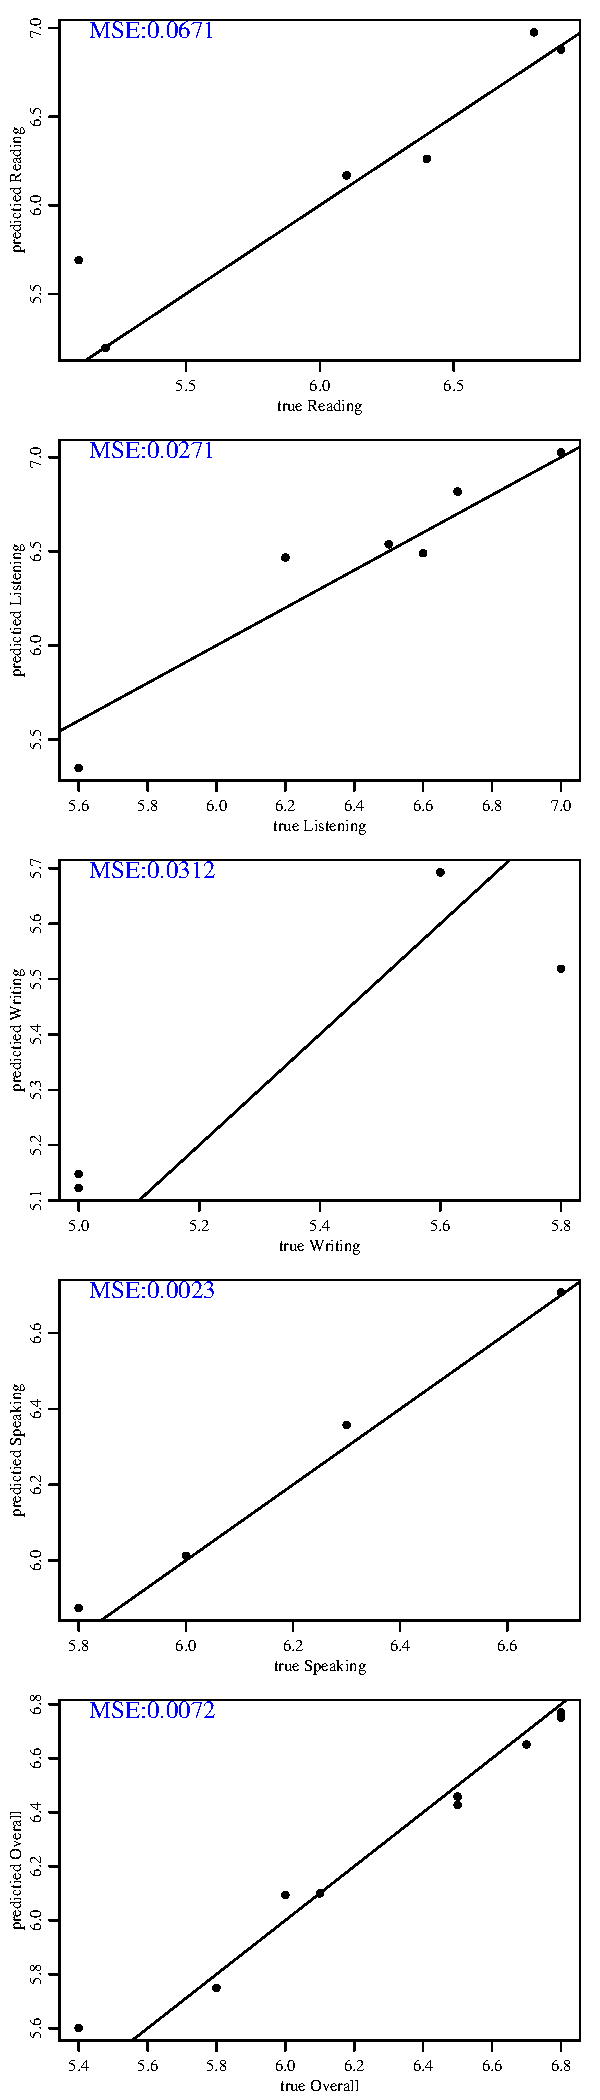
\includegraphics[height=.85\textheight]{pic/0.15/EM_PredvsTrue.pdf}
    \caption{EM algorithm}
    \label{fig:0.15-empvt}
\end{subfigure}
%\hfill
\begin{subfigure}{0.4\textwidth}
    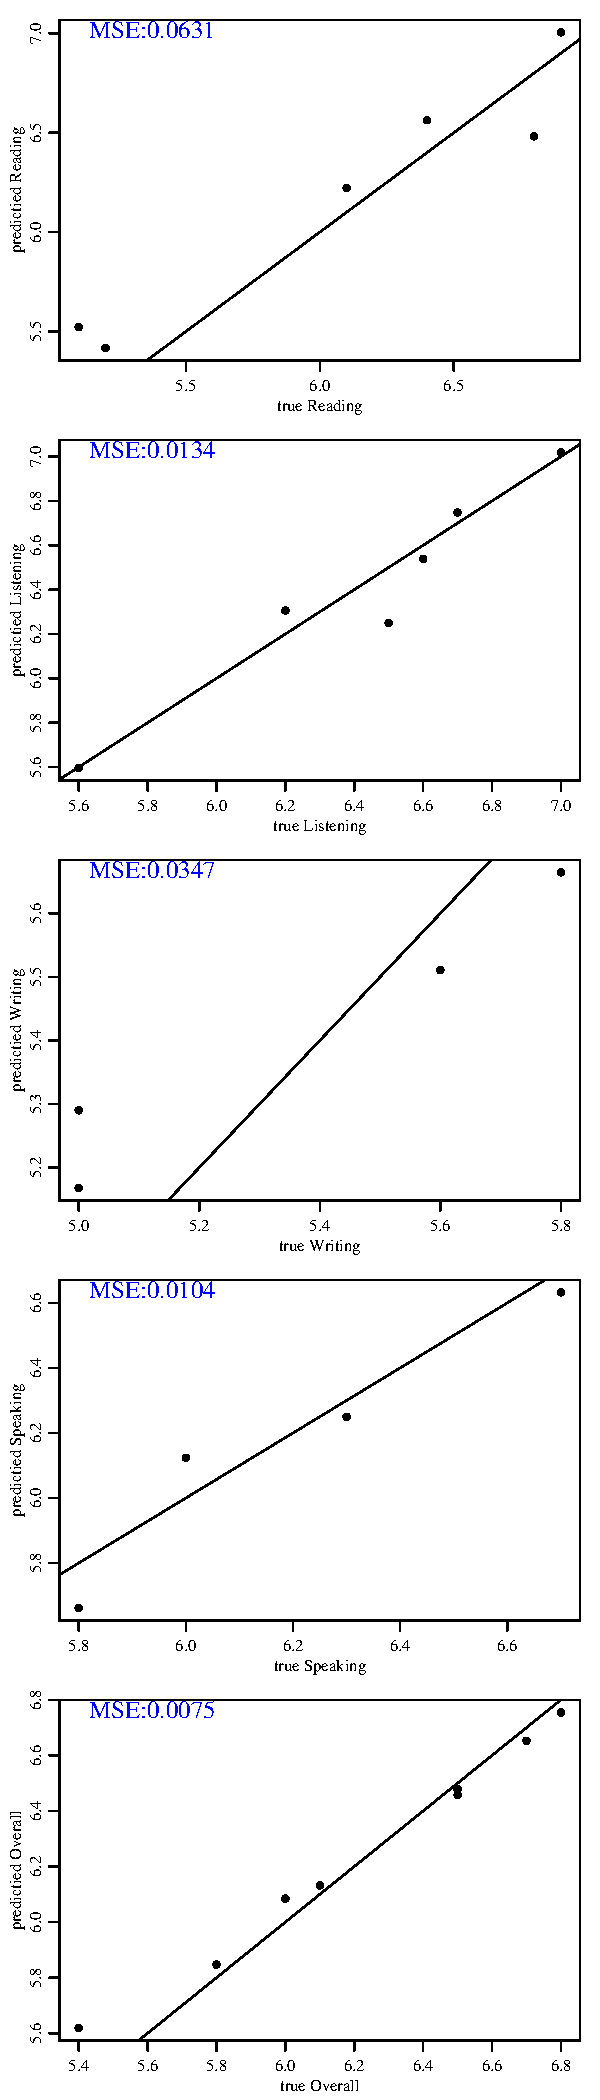
\includegraphics[height=.85\textheight]{pic/0.15/Gibbs_PredvsTrue.pdf}
    \caption{Gibbs sampling method}
    \label{fig:0.15-gibbspvt}
\end{subfigure}
        
\caption{Prediction vs True value}
\label{fig:0.15-pvt}
\end{figure}

\begin{figure}[htbp]
	\centering
	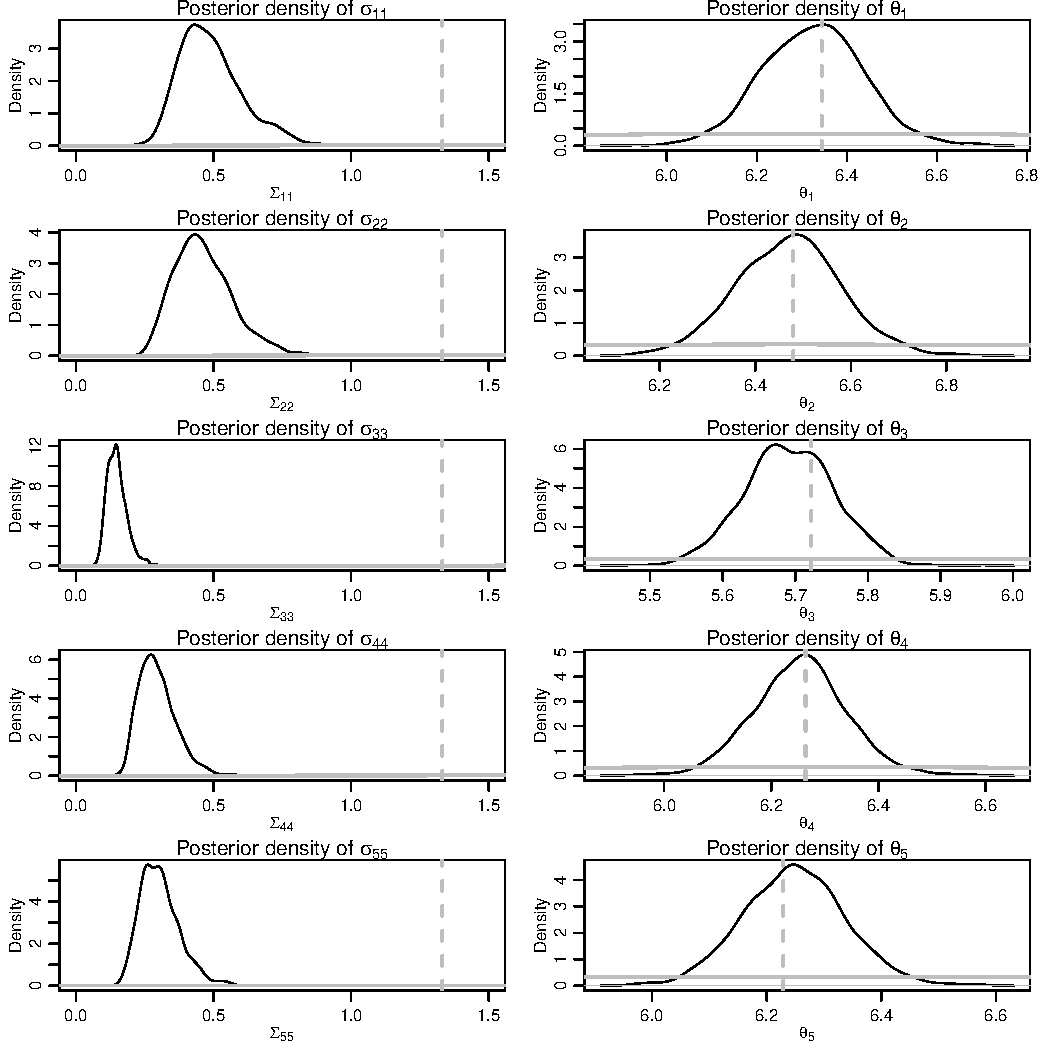
\includegraphics[width=.9\textwidth]{pic/0.15/Posterior_vs_Prior.pdf}
	\caption{The posterior (and prior) distribution of $\sigma_{j, j}$ (left) and $\theta_j$ (right). Posterior distribution is ploted in black, and prior distribution is ploted in gray. The vertical dashed line marks the initial value for prior.}
	\label{fig:0.15-Posterior_vs_Prior}
\end{figure}

\newpage
\subsubsection{20\% of missing data}
\begin{figure}[h!]
\centering
\begin{subfigure}{0.4\textwidth}
    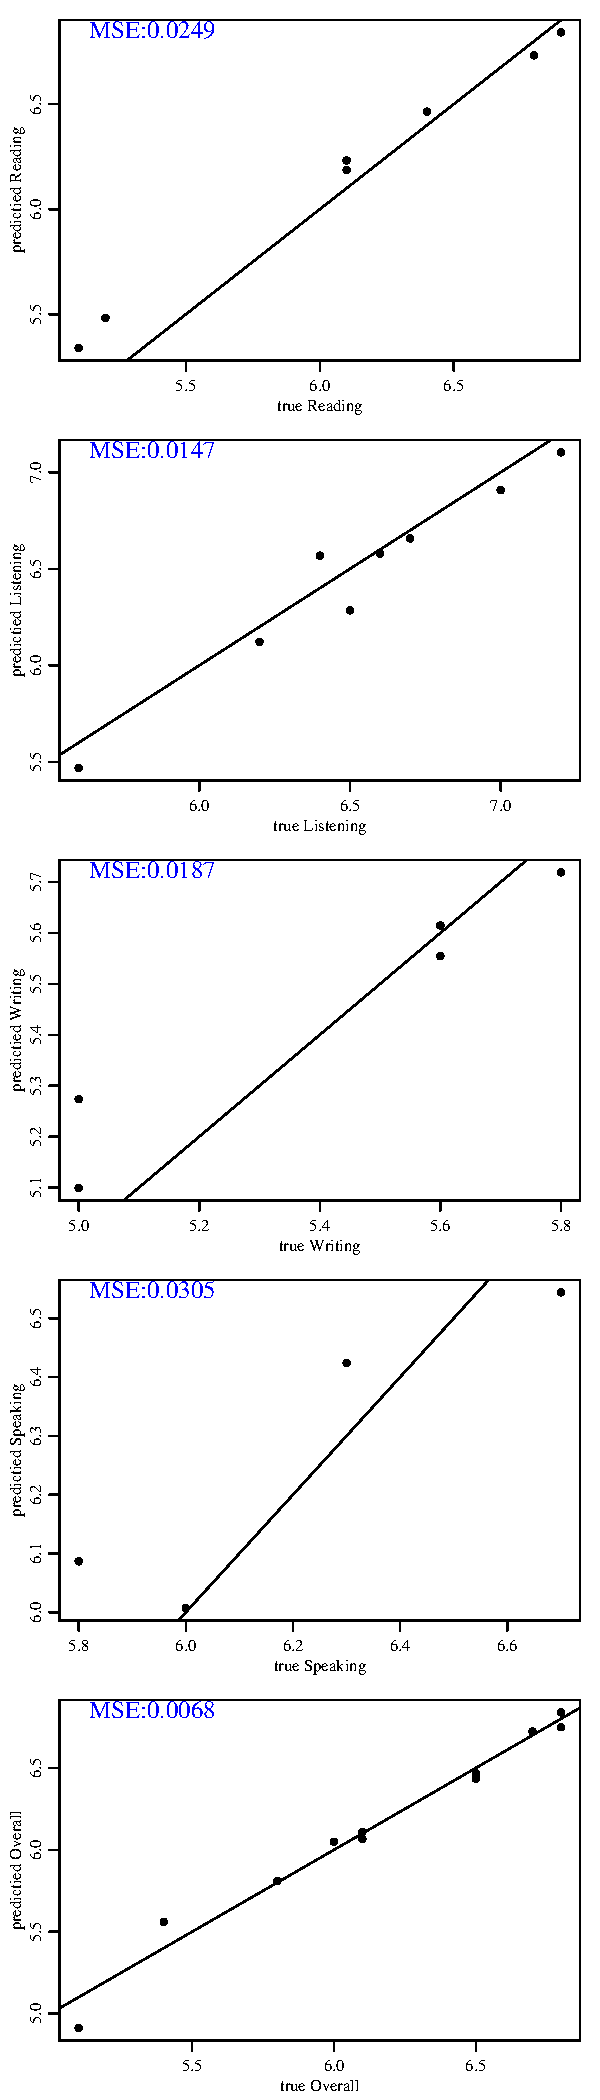
\includegraphics[height=.85\textheight]{pic/0.20/EM_PredvsTrue.pdf}
    \caption{EM algorithm}
    \label{fig:0.20-empvt}
\end{subfigure}
%\hfill
\begin{subfigure}{0.4\textwidth}
    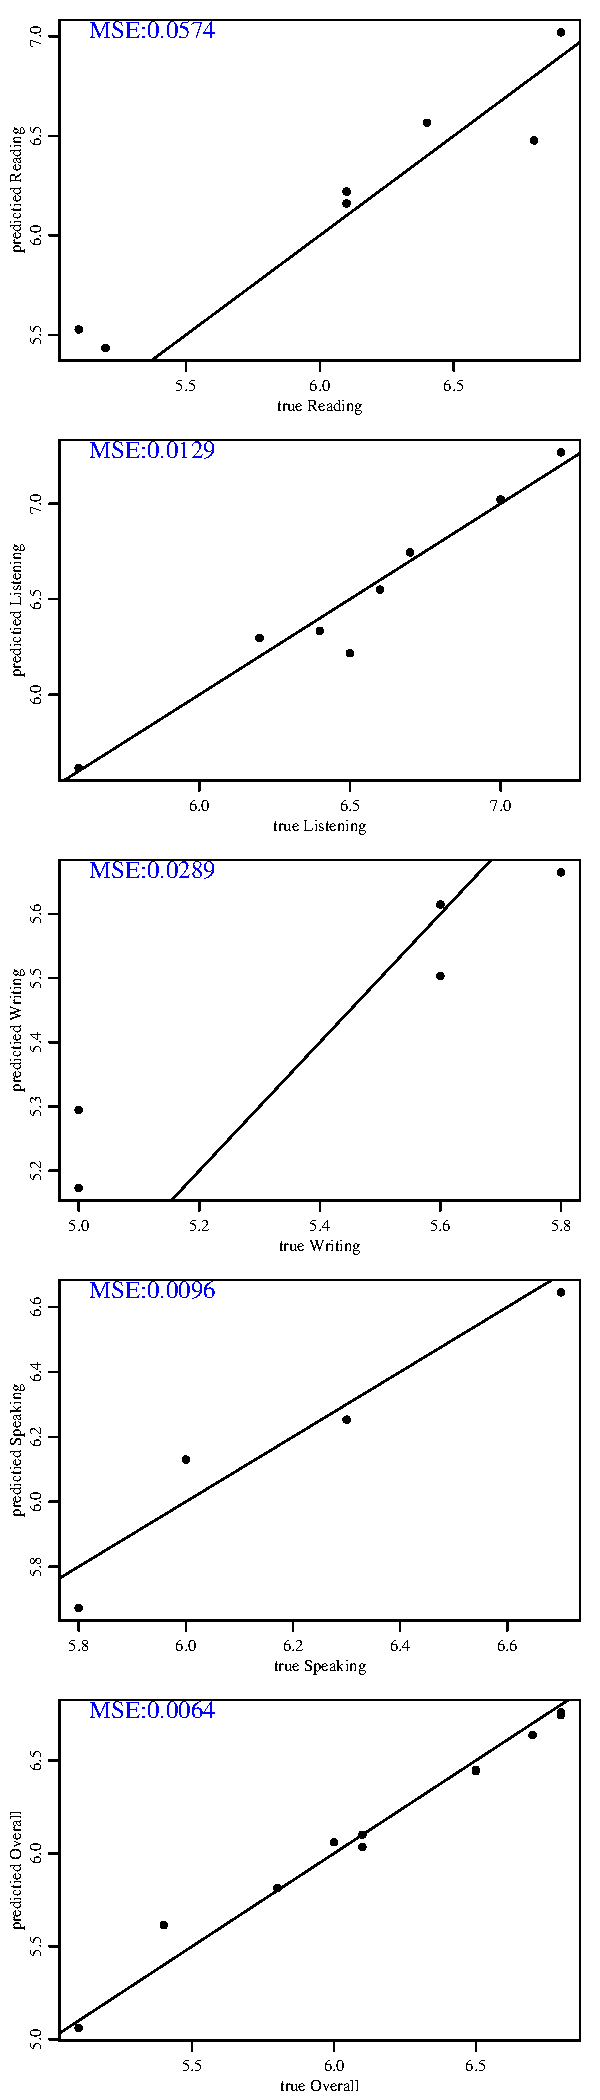
\includegraphics[height=.85\textheight]{pic/0.20/Gibbs_PredvsTrue.pdf}
    \caption{Gibbs sampling method}
    \label{fig:0.20-gibbspvt}
\end{subfigure}
        
\caption{Prediction vs True value}
\label{fig:0.20-pvt}
\end{figure}

\begin{figure}[htbp]
	\centering
	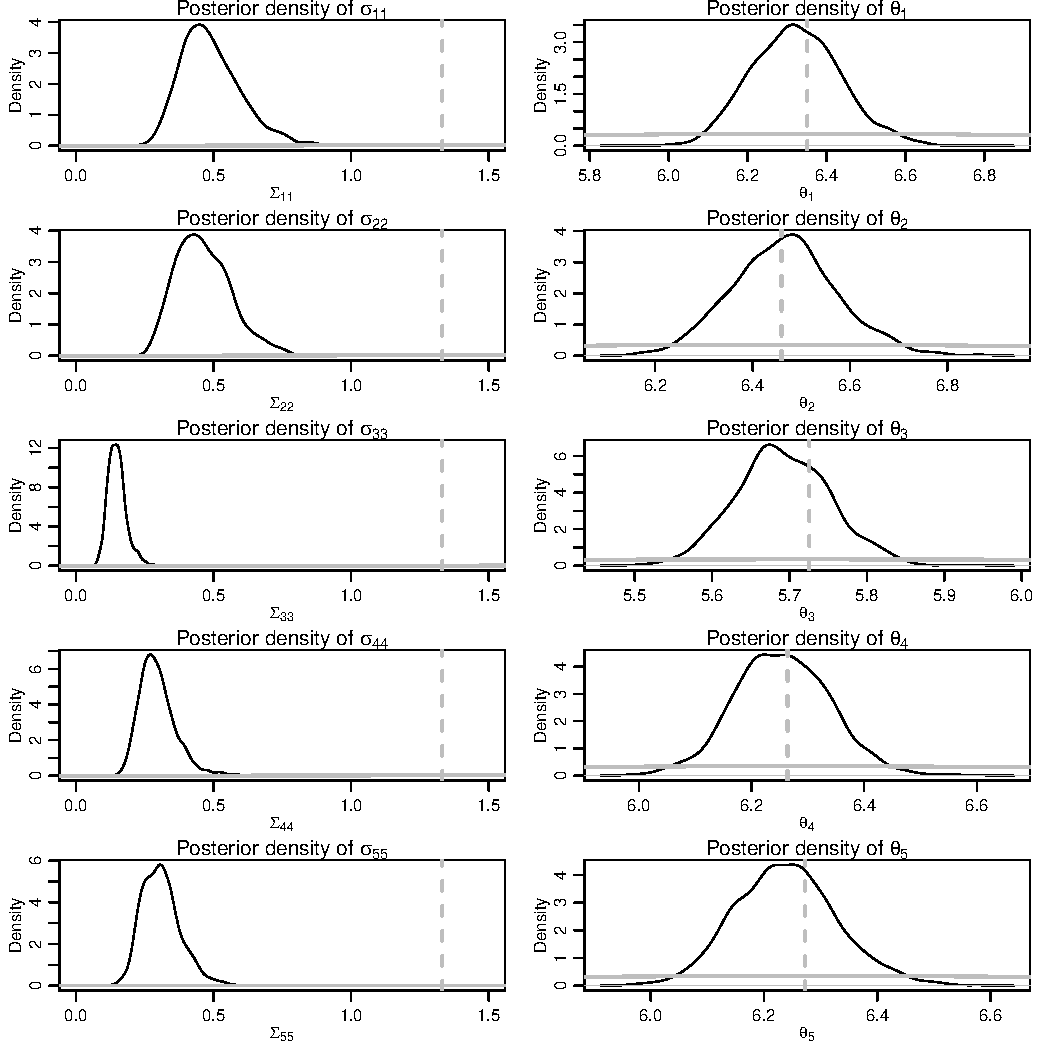
\includegraphics[width=.9\textwidth]{pic/0.20/Posterior_vs_Prior.pdf}
	\caption{The posterior (and prior) distribution of $\sigma_{j, j}$ (left) and $\theta_j$ (right). Posterior distribution is ploted in black, and prior distribution is ploted in gray. The vertical dashed line marks the initial value for prior.}
	\label{fig:0.20-Posterior_vs_Prior}
\end{figure}

\newpage
\subsubsection{25\% of missing data}
\begin{figure}[h!]
\centering
\begin{subfigure}{0.4\textwidth}
    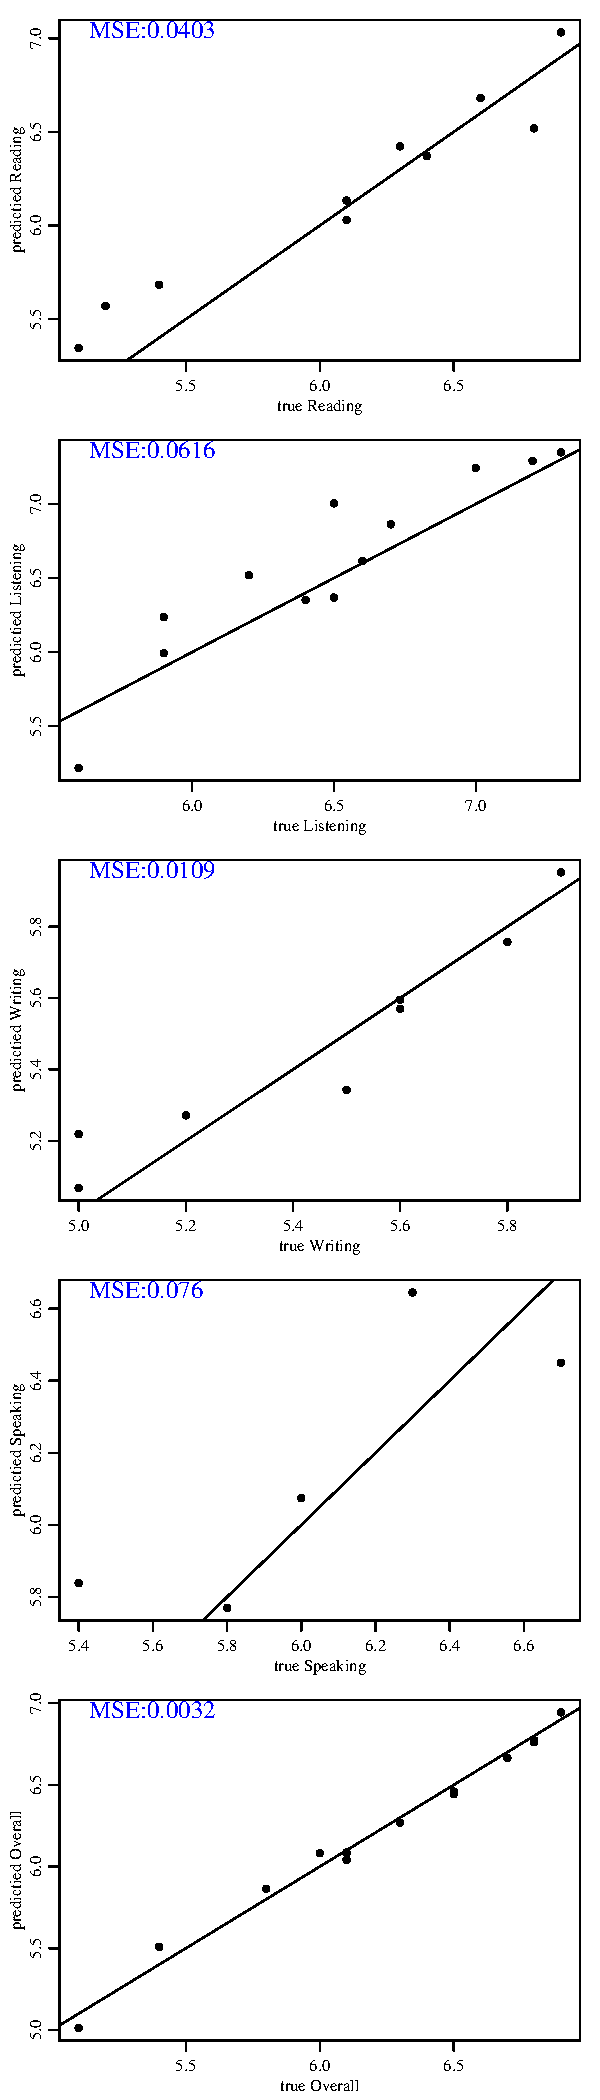
\includegraphics[height=.85\textheight]{pic/0.25/EM_PredvsTrue.pdf}
    \caption{EM algorithm}
    \label{fig:0.25-empvt}
\end{subfigure}
%\hfill
\begin{subfigure}{0.4\textwidth}
    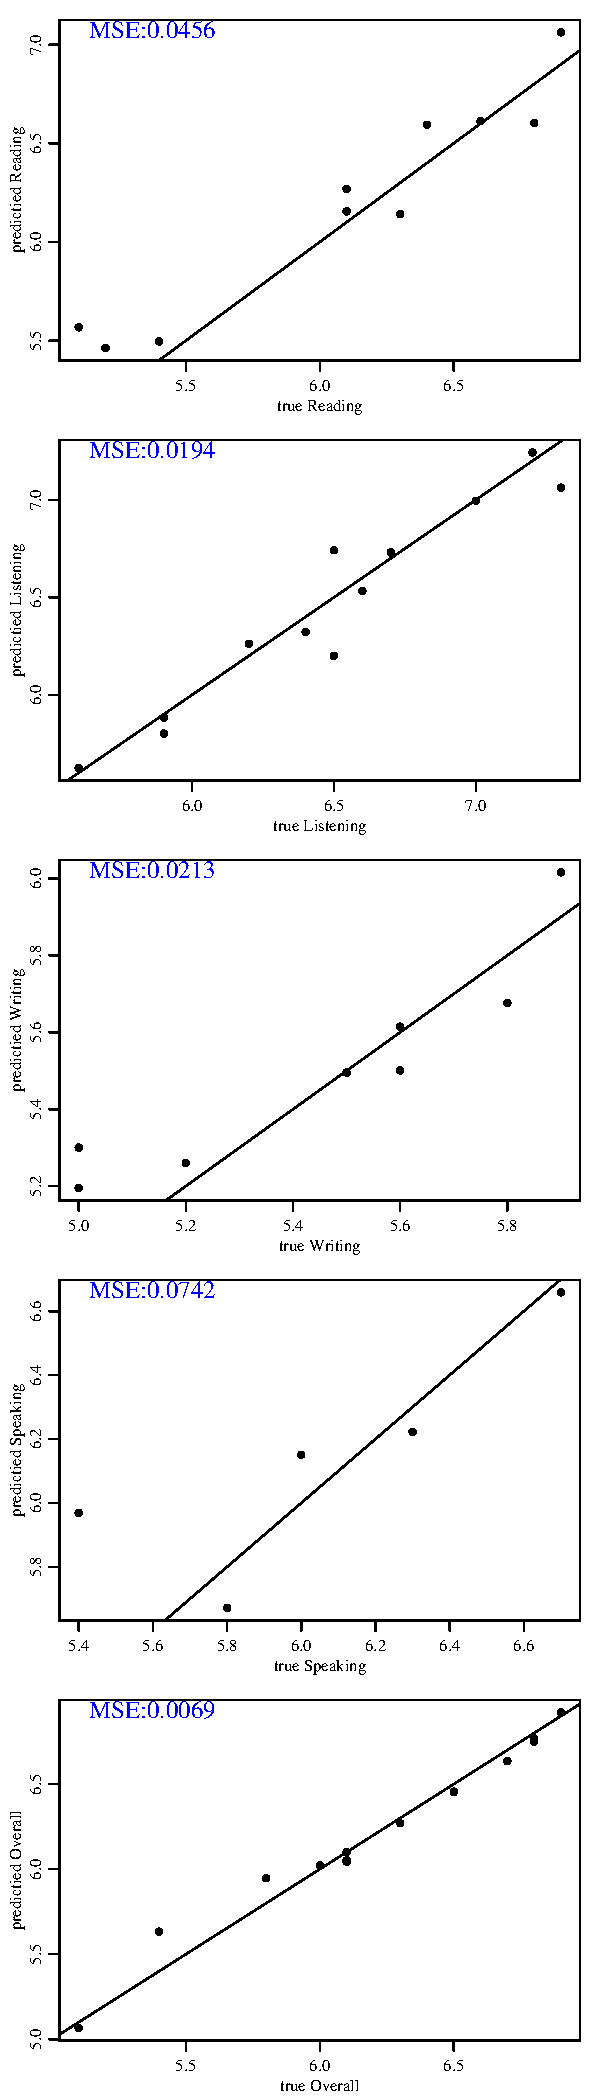
\includegraphics[height=.85\textheight]{pic/0.25/Gibbs_PredvsTrue.pdf}
    \caption{Gibbs sampling method}
    \label{fig:0.25-gibbspvt}
\end{subfigure}
        
\caption{Prediction vs True value}
\label{fig:0.25-pvt}
\end{figure}

\begin{figure}[htbp]
	\centering
	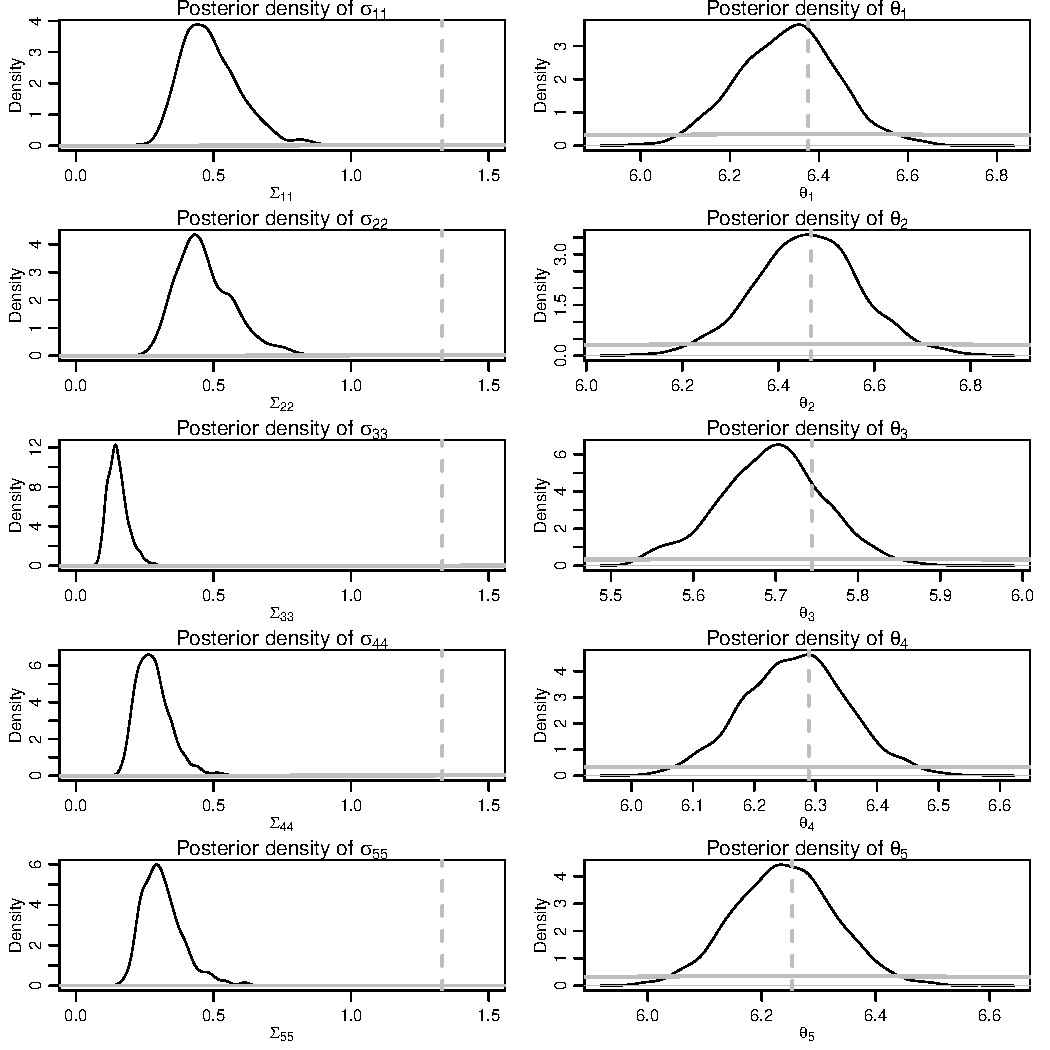
\includegraphics[width=.9\textwidth]{pic/0.25/Posterior_vs_Prior.pdf}
	\caption{The posterior (and prior) distribution of $\sigma_{j, j}$ (left) and $\theta_j$ (right). Posterior distribution is ploted in black, and prior distribution is ploted in gray. The vertical dashed line marks the initial value for prior.}
	\label{fig:0.25-Posterior_vs_Prior}
\end{figure}

\newpage
\subsubsection{30\% of missing data}
\begin{figure}[h!]
\centering
\begin{subfigure}{0.4\textwidth}
    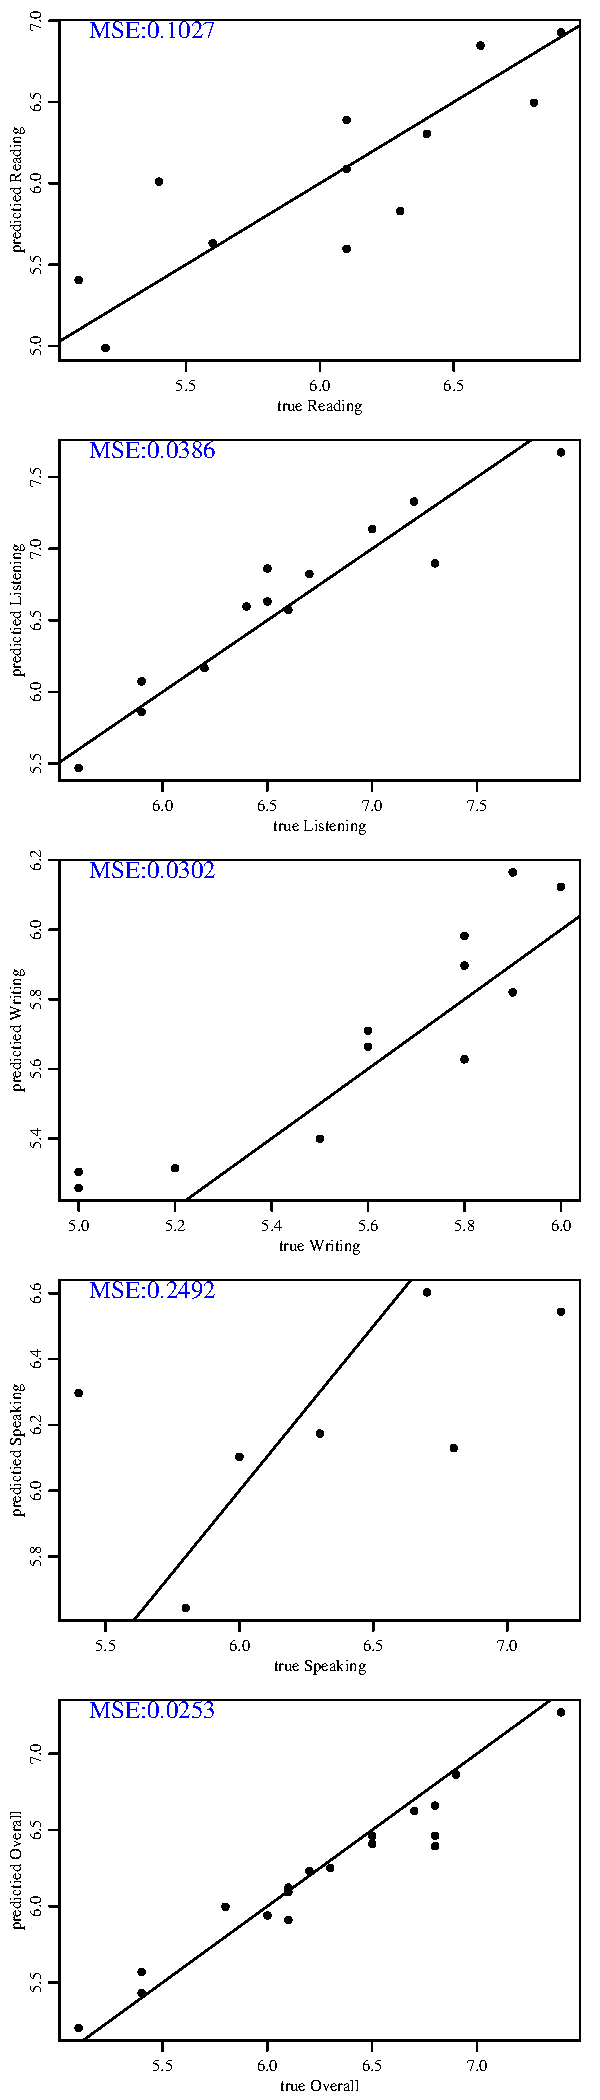
\includegraphics[height=.85\textheight]{pic/0.30/EM_PredvsTrue.pdf}
    \caption{EM algorithm}
    \label{fig:0.30-empvt}
\end{subfigure}
%\hfill
\begin{subfigure}{0.4\textwidth}
    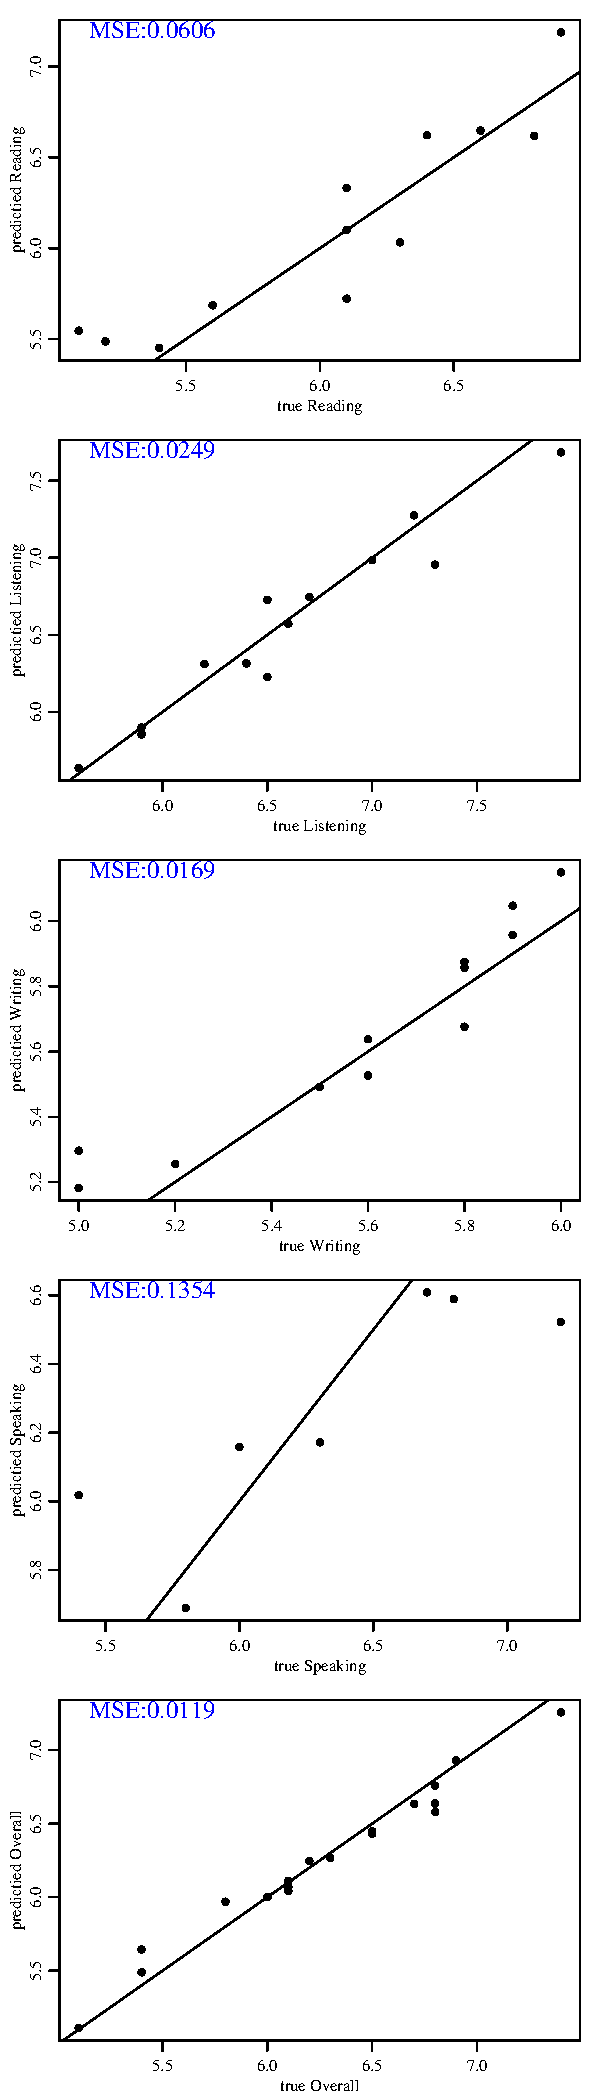
\includegraphics[height=.85\textheight]{pic/0.30/Gibbs_PredvsTrue.pdf}
    \caption{Gibbs sampling method}
    \label{fig:0.30-gibbspvt}
\end{subfigure}
        
\caption{Prediction vs True value}
\label{fig:0.30-pvt}
\end{figure}

\begin{figure}[h!]
	\centering
	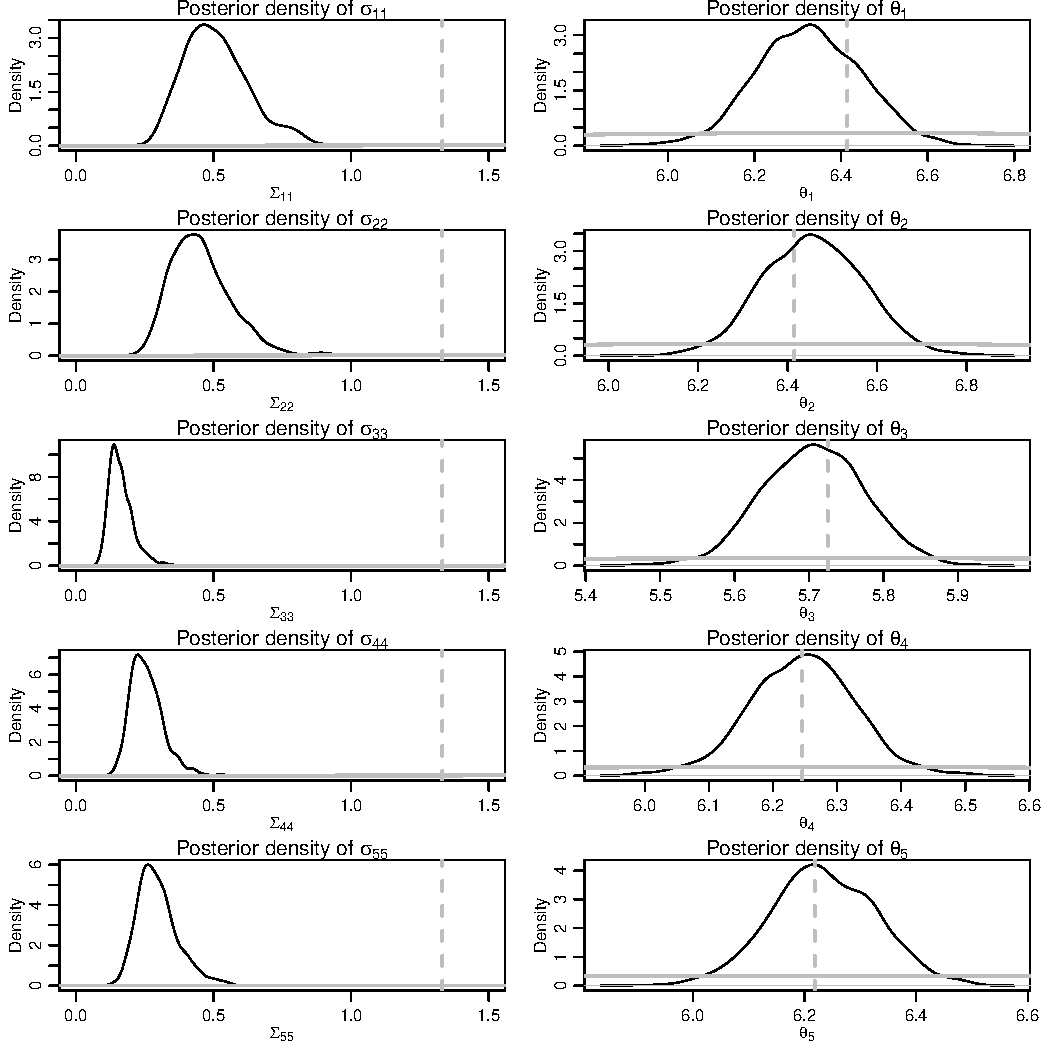
\includegraphics[width=.9\textwidth]{pic/0.30/Posterior_vs_Prior.pdf}
	\caption{The posterior (and prior) distribution of $\sigma_{j, j}$ (left) and $\theta_j$ (right). Posterior distribution is ploted in black, and prior distribution is ploted in gray. The vertical dashed line marks the initial value for prior.}
	\label{fig:0.30-Posterior_vs_Prior}
\end{figure}
\end{document}
